\documentclass[final]{siamltexmm}
\documentclass[10pt,a4paper]{article}

\usepackage{graphicx}
\usepackage{algorithm}
\usepackage{algorithmic}

\usepackage[demo]{graphicx}
\usepackage{subfig}

\newcommand{\pe}{\psi}
\def\d{\delta} 
\def\ds{\displaystyle} 
\def\e{{\epsilon}} 
\def\eb{\bar{\eta}}  
\def\enorm#1{\|#1\|_2} 
\def\Fp{F^\prime}  
\def\fishpack{{FISHPACK}} 
\def\fortran{{FORTRAN}} 
\def\gmres{{GMRES}} 
\def\gmresm{{\rm GMRES($m$)}} 
\def\Kc{{\cal K}} 
\def\norm#1{\|#1\|} 
\def\wb{{\bar w}} 
\def\zb{{\bar z}} 

% some definitions of bold math italics to make typing easier.
% They are used in the corollary.

\def\bfE{\mbox{\boldmath$E$}}
\def\bfG{\mbox{\boldmath$G$}}

\title{Computational Machine Learning Homework4}
\author{Yun-shao Sung\thanks{\tt yss265@nyu.edu}
        \and Hung-Ting Wen\thanks{\tt htw230@nyu.edu}}

\begin{document}
\maketitle

\begin{abstract}
This document served as the purpose of answering qestions from homework assignment, and also conclude the experiment observations.
\end{abstract}

\pagestyle{myheadings}
\thispagestyle{plain}


\section{Introduction \& Background}
Our purpose of this project is to build a learning machine that can distinguish between different music genres.  Music genre classification has never been an easy task, even for human.  Different chords, beats, and tonality can change the way people perceive about a song, even with slightest differences.  Therefore, the biggest challenge for us is how to extract and distinguish those meaningful differences from signals.

Hence, our project focused on feature extraction using different approaches on signals.  We started with re-creating results of 2nd-order scattering \cite{mgc} , for which we have accuracy of 79\%, which is close to the results of our reference paper.

The data set we are using is GTZAN Music Genre Collection \cite{data} , which parallels with our reference paper and many other similar works.  This data set contains 10 genres, where each genre has 100 tracks in it.

However, we faced memory usage problem when running 2nd-order scattering.  Given a clip of signals with size of 50000, after 2nd-order scattering it will become size of $670 \times 50000$, and it's only on clip.  We have 10 clips per song, and there has 1000 songs in total.

Inspired by 2nd-order scattering, we moved on to design several different appraoches, focused on extracting different but yet meaningful signals from raw data, as if it's a layered material and we are trying to break down its components.  With these approaches, memory usage is not growing that fast and thus our experimental obstacle was solved.  Hence, we moved on to focus on improving correctness.  That is, verify whether our feature extraction approaches make sense or not through experimental results on predictin accuracy.

\begin{figure}[ht]
  \begin{center}
    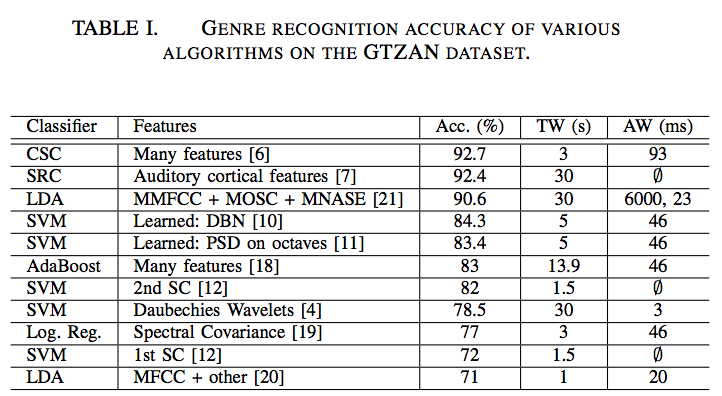
\includegraphics[scale=0.7]{../fig/refAccr.png}
  \end{center}
\end{figure}

From Table I. we can see various experiment results with different classifiers and different ways of featuer extraction.  Our experiment results didn't reach the result on top of list.  Part of reason is because we didn't try to use some fancy classifiers.  Instead, since we focused on feature extraction, we use only KNN and SVC as our classifiers in order to see a comparable results.  As a result, our prediction accuracies are concentrated around 70\% to 75\% and we hit 79\% often.  Robustness became one of our major results.

\section{Baseline Approaches}
To have our baseline approaches reaching similar accuracy as the previous finding, we have implemented some methods trying to reach the goal, and also trying to test our hypothesis. First of all is the interpretation of MFCC product. The MFCC product will be the shape of (n\_mfcc, time), which n\_mfcc is the number of mel-frequency and we set as 20, and time this time frame of the input clip signal. Then, as the instinct from previous experiment, we transpose MFCC product to the shape of (time, n\_mfcc) which is transforming the meaning of feature representation of each mel-frequency over time to feature representation of each time moment in the clip over time mel-frequency. Althought this transpose will yield better accracucy, the further interprestation is yet unsure. We are not sure whether we should treat transposed-MFCC product as multi points in n\_mfcc-dim space, or treat transposed-MFCC product as one point in $time \times n\_mfcc$-dim space.
\\The second question is about the VLAD. The idea of the VLAD descriptor is to accumulate, for each visual word $c_{i}$, the differences x-$c_{i}$ of the vectors x assigned to $c_{i}$:
\begin{equation}
c_{i, j} = \sum\limits_{x such that NN(x)=c_{i}} x_{i}-c_{i,j}
\end{equation}
where $x_{i}$ and $c_{i,j}$ respectively denote the jth component of the descriptor x considered and of its corresponding visual word $c_{i}$. We was wondering what if we sum up all the result into just d-dimension instead of the original VLAD representation $D=k\times d$, where k and d are the number of centroids and dimension of each centroid. Therefore, we named these two VLAD methods as Sum VLAD and Concatenate VLAD, and due to high dimension of Concatenate VLAD, we then perforemed PCA with whitening for dimension reduction.
\\\\As the results of the questions mentioned previously, we performed the folloing appraoches to reach the questions:
\\ 1. multi points MFCC + Kmeans + Sum VLAD + k nearest neighbor
\\ 2. multi points MFCC + Kmeans + Sum VLAD + SVC
\\ 3. one point MFCC + Kmeans + Sum VLAD + SVC
\\ 4. multi points MFCC + Kmeans + Concatenate VLAD + PCA + k nearest neighbor
\\ 5. multi points MFCC + Kmeans + Concatenate VLAD + PCA + SVC
\\ 6. one points MFCC + Kmeans + Concatenate VLAD + PCA + SVC
\begin{figure}%
    \centering
    \subfloat[Baseline method 5]{{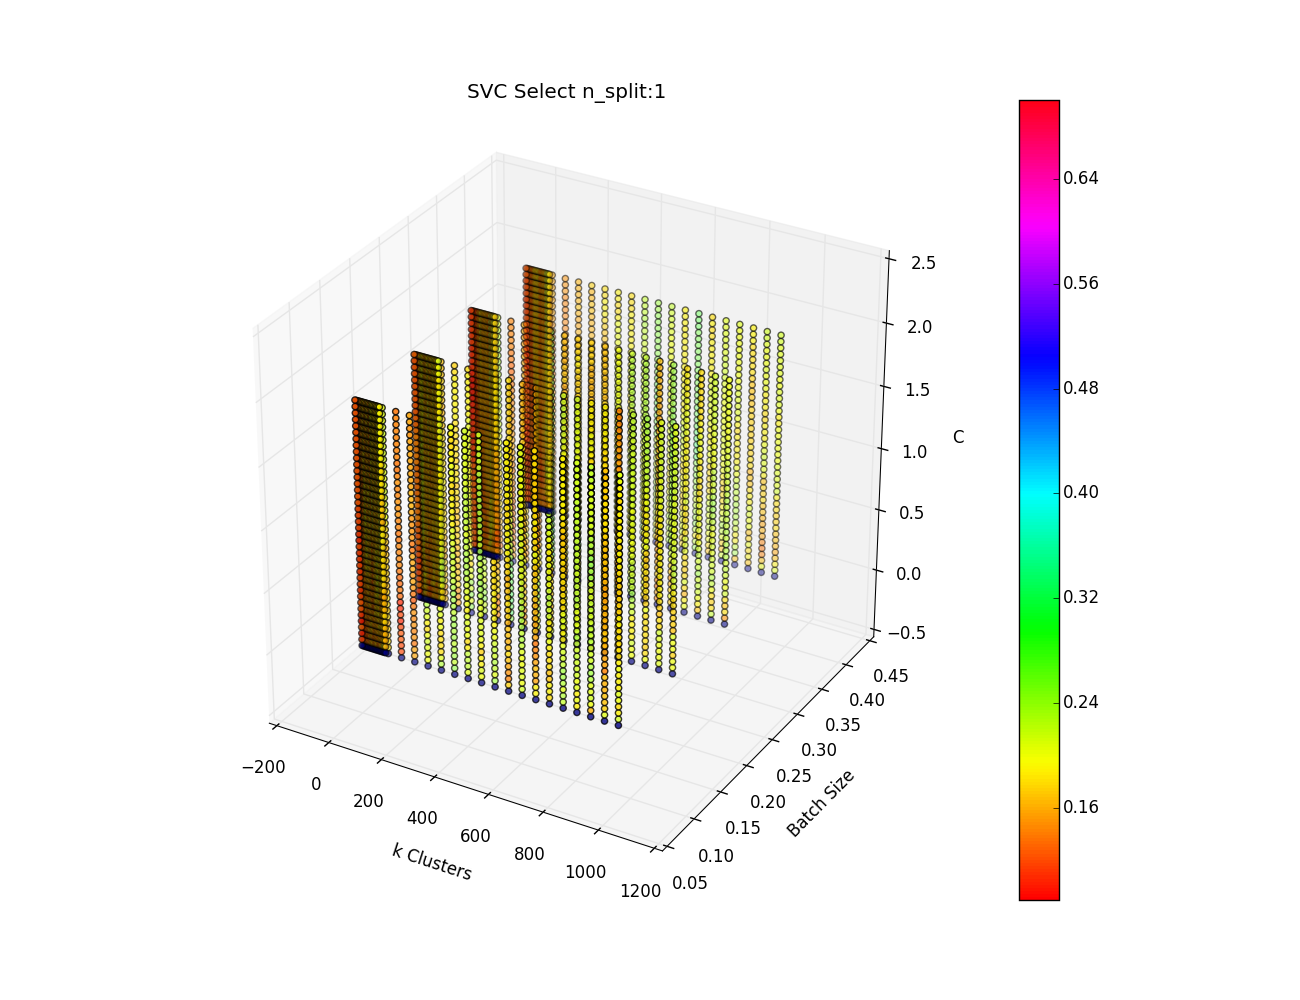
\includegraphics[width=5cm]{../fig/svcSplit1_svcNewVLAD200Iter.png} }}%
    \qquad
    \subfloat[Feature extraction method 3]{{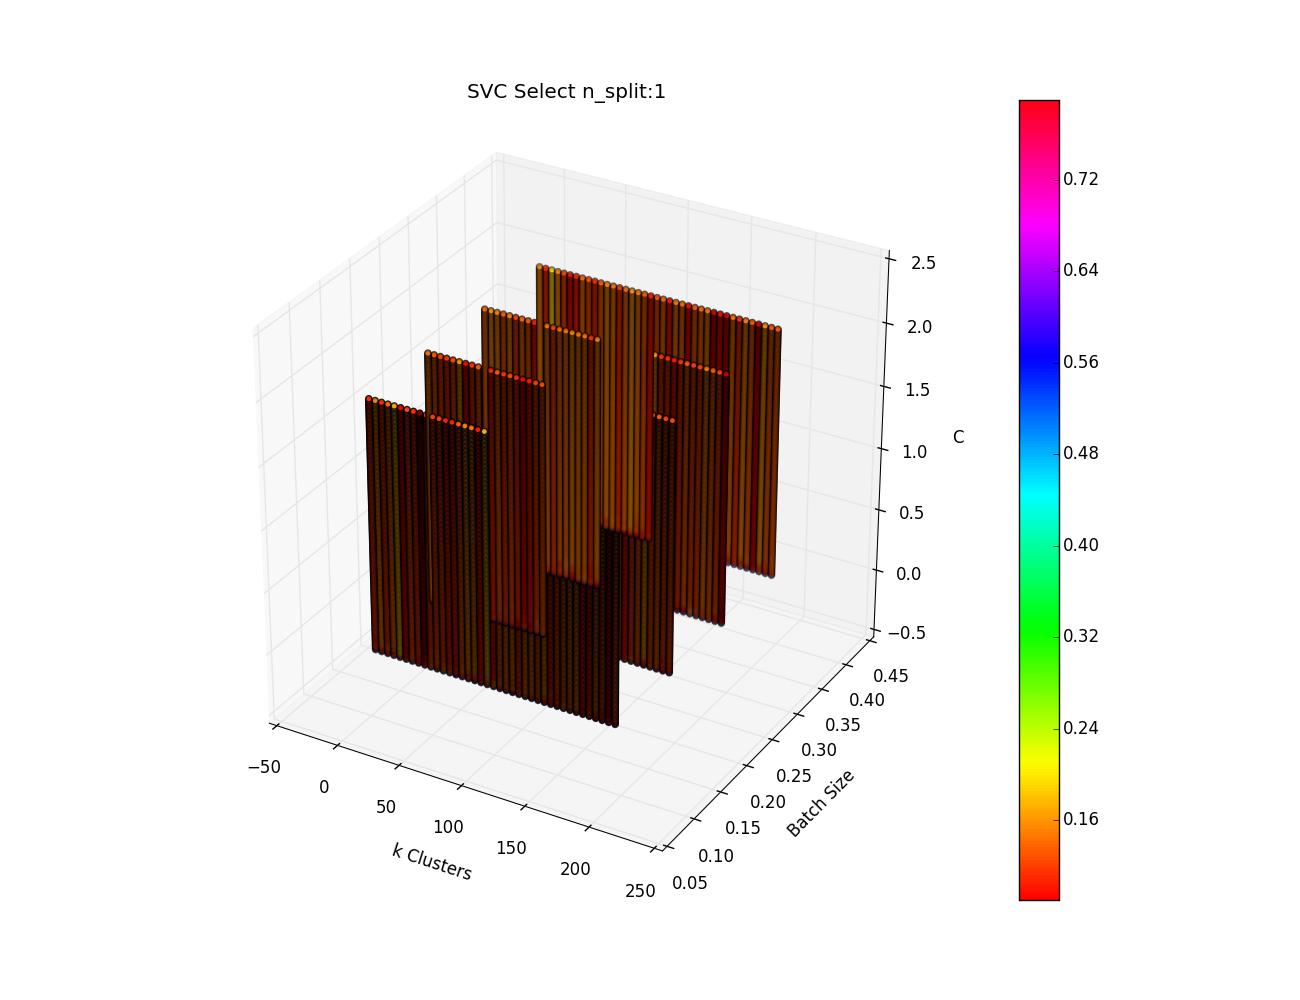
\includegraphics[width=5cm]{../fig/svcFlatSplit1_ScatterHPMFCCNewVLAD.png} }}%
    \caption{Best accuracy from baseline and new extraction method}%
    \label{fig:example}%
\end{figure}

As comparing method 1 and 2, we noticed generally SVC has better accuracy than KNN, but also at the cost of efficiency. This may due to the properity that SVC is using 1-vs-1 scheme for $n\_classes\times(n\_classes-1)/2$ times, which maybe more delicate than KNN. We have also tested the LinearSVC method, which is 1-vs-rest scheme. Generally speaking, the accuracy of LinearSVC is still better than KNN and slightly lower than SVC.

By having the result from method 3 and compare to method 2, we noticed we cannot get any furthre improvement from method 3, and even the accuracy is decreased. This phenomenon is getting even worse when comparing the results from method 5 and 6. Therefore, we can clearly see treating the MFCC product as one point is definitely not a good method, and the possible explaination for this is probably due to we are fixing the sequencing meaning of feature representation into fixed order. For example a clip from Jazz genre may have the component of drum, guitar, and bass, and MFCC product gives us the features quantification at each time points. As we concatenate them with the fixed order, we are like telling the classifier the feature with this is order is belong to certain genre. However, the order of drump-guitar-bass or guitar-bass-drump should be equally considered as Jazz.

As comparing the method4 versus method1 and method5 versus method2, we can see the accuracy increased, especially in method5. Our centroids are obtained from the Kmeans of our implementation with Kmean++ for initialization and maxIter=200 as stopping criteria. Then our cancatenate VLAD method is the accumulation of measurement of each residuals, which defined as the vecter differences between each feature points and center, and then instead of sum up all vectors, here we concatenate each residuals. This method gave us a significant accuracy improvement, and is very likely due to concatenate each residuals at the same level will keep the strong feature while still save the minority feature representations. For example, if now this song which belong to Jazz has strong drum-related feature but also contains some guitar and bass feature that are not strong but yet representative enough, summing them all up like what we did in method 1-3 will easily loss those minority features. An abstraction metaphor for this idea, which hugely inspired our next new feature extraction method, is like a onion. During each step of our pipeline, we can either treat the onion as a whole, which we might not know this onion has multi-layers or probably we even don't know know this is a onion because it looks like a apple, or we can peeling each of the layer out and concatenate each layer together. The peeling process will give us better understanding about this onion.

In summary regarding to our current progress, which the pipeline described in method 5,our MFCC can reach to the accuracy of 70\%, which is comparible to previous finding.

\begin{table}[h!]
\centering
  \begin{tabular}{ l || c | r }
    \hline
    Method Ids & Accuracy (\%) \\ \hline \hline
    Method 1 & 48 \\ \hline
    Method 2 & 58 \\ \hline
    Method 3 & 56 \\ \hline
    Method 4 & 50 \\ \hline
    Method 5 & 70 \\ \hline
    Method 6 & 33 \\ \hline
    \hline
  \end{tabular}
\caption{Methods of each baseline approaches and its corresponding accuracy.}
\label{table:1}
\end{table}

\section{New Feature Extraction Approaches}
As our result from baseline approaches (best 70\%) yields is comparable to previouse finding using MFCC (best 71\%), we also, based on the fundation of best baseline approach, experimentally invent new methods trying to further improve the best accuracy as well as the robustness of parameter searching, and here we mainly focus on the improvement of feature extraction. In additional to regular mfcc, librosa provides harmonic and percussive seperation (librosa.effects.hpss), which the underline mechanism is the STFT-HPSS-ISTFT pipeline, and it ensures that the output waveforms have equal length to the input signal. Secondly, we are trying to use librosa delta method (librosa.feature.delta) to capture the first and second derivative information from harmonic and percussive signal. As we mentioned from previous baseline method, concatenating MFCC product and treating it as one point is fixing the signal sequecial meaning which will limit the freedom the classification. However, the signal transition at every monent might hiding clear feature representation, and, therefore, taking the signal derivative and treat it as feature representation points might be a useful method. The final approach is the scattering of HPSS, and this idea is probably inspired by the switch of Sum VLAD to Concatenate VLAD mentioned previously. We noticed even signal being splited to harmonic and percussive parts, there are still plenty of residue signal in each splits. For example, although being removed significantly, there are still noticable percussive components in the harmonic split, and vise versa. Therefore, here we performed second order HPSS scattering as the new feature extraction method.

\begin{algorithm}[htb]
  \caption{HPSS Scattering}
  \label{algo:SC}
\begin{algorithmic}[1]
  \FOR{$eachClip \in Song$}
    \STATE y\_h1, y\_p1 = librosa.effects.hpss(y)
    \STATE y\_h2, y\_p2 = librosa.effects.hpss(y\_h1)
    \STATE y\_h3, y\_p3 = librosa.effects.hpss(y\_p1)
    \STATE y\_h4, y\_p4 = librosa.effects.hpss(y\_h2)
    \STATE y\_h5, y\_p5 = librosa.effects.hpss(y\_p2)
    \STATE y\_h6, y\_p6 = librosa.effects.hpss(y\_h3)
    \STATE y\_h7, y\_p7 = librosa.effects.hpss(y\_p3)
    \STATE map(MFCC, [y\_h1, y\_p1, y\_h2, y\_p2, y\_h3, y\_p3, y\_h4, y\_p4, y\_h5, y\_p5, y\_h6, y\_p6, y\_h7, y\_p7])
  \ENDFOR
\end{algorithmic}
\end{algorithm}
Below are our new approaches:
\\ 1. HPSS + MFCC + method 5 in baseline approach
\\ 2. HPSS w/ 1st delta w/ 2nd delta + MFCC + method 5 in baseline approach
\\ 3. 2nd HPSS scattering + MFCC + method 5 in baseline approach
\\

From the original method mentioned in baseline approaches, now our method 1 can further reached to 77\% of accuracy. As shown in figure 4.1, we noticed the harmonic and percussiv seperation is essential as we make the spectrogram plot of each parts. From the spectrogram plot of original clip, certain time period in original clip looks just like normal but these peroids actually existing noticable differences between harmonic and percussive parts. Just like the onion metaphor mentioned previously, we believe peeling off the original clip and contcate each of parts followed by MFCC will give us more feature representation to understand this song. As the result of this approach, in the improvement of this approach not only increase the max accuracy to 77\%, but also improve the robustness of the search space. As we can see the row 2 in figure 4.3, the major peak of the search space now significantly shift from original accuracy of 50\% to 65\%. This implies this new feature extraction method can potentially release the computation time and guarantee a better accuracy.

\begin{figure}[!ht]
  \centering
    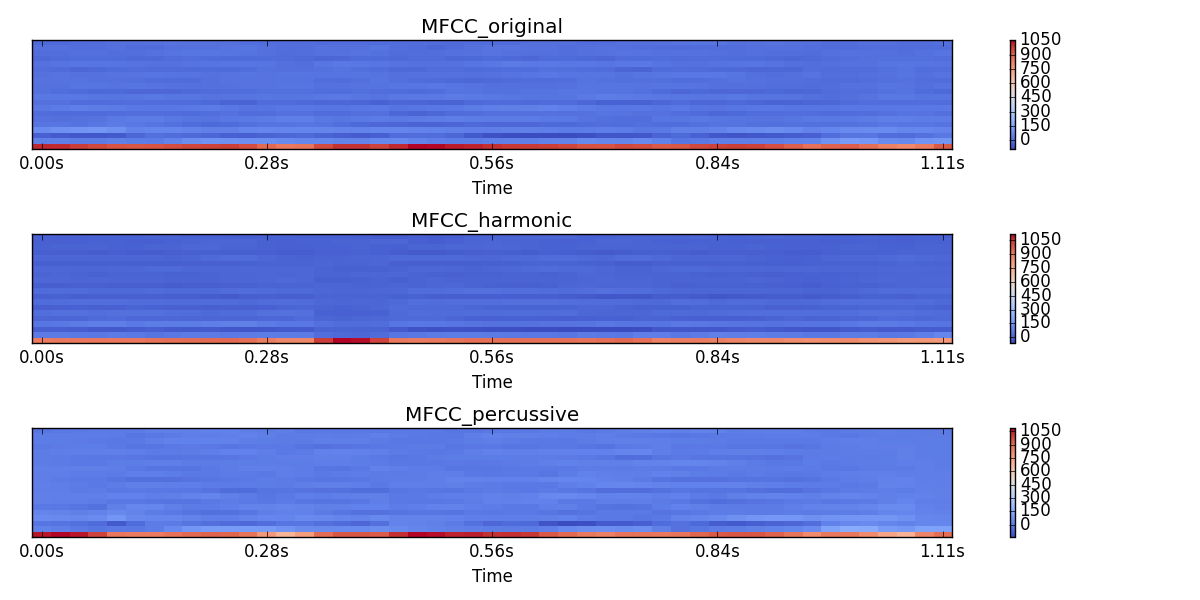
\includegraphics[width=0.7\textwidth]{../fig/harmonic_percussiv_mfcc_nolog.png}
  \caption{MFCC spectrogram of original clip, harmonic, and percussiv parts}
\end{figure}

\\In figure 4.2, not just the differences in harmonic and percussive parts of original song clip, we can also see the apparent difference when we take 1-order and 2-order of feature.delta. Instead of the original clip and its derivative here we keep only the harmonic and percussive parts and its 1-order and 2-order derivative. Therefore, the feature point of each song clip will be 6 times more than baseline method 5. Although we are not sure whether it's meaningful to keep the derivative information, in figure 4.3 row 3, it turns out the result as well as its robustness are quite improved when comparing to the best baseline method. As the definition of derivative is taking the transient difference in a tiny time interval and turns out it looks like a meaningful representation, we assume the signal transition at each monent might still be a good representation of song.

\begin{figure}[!ht]
  \centering
    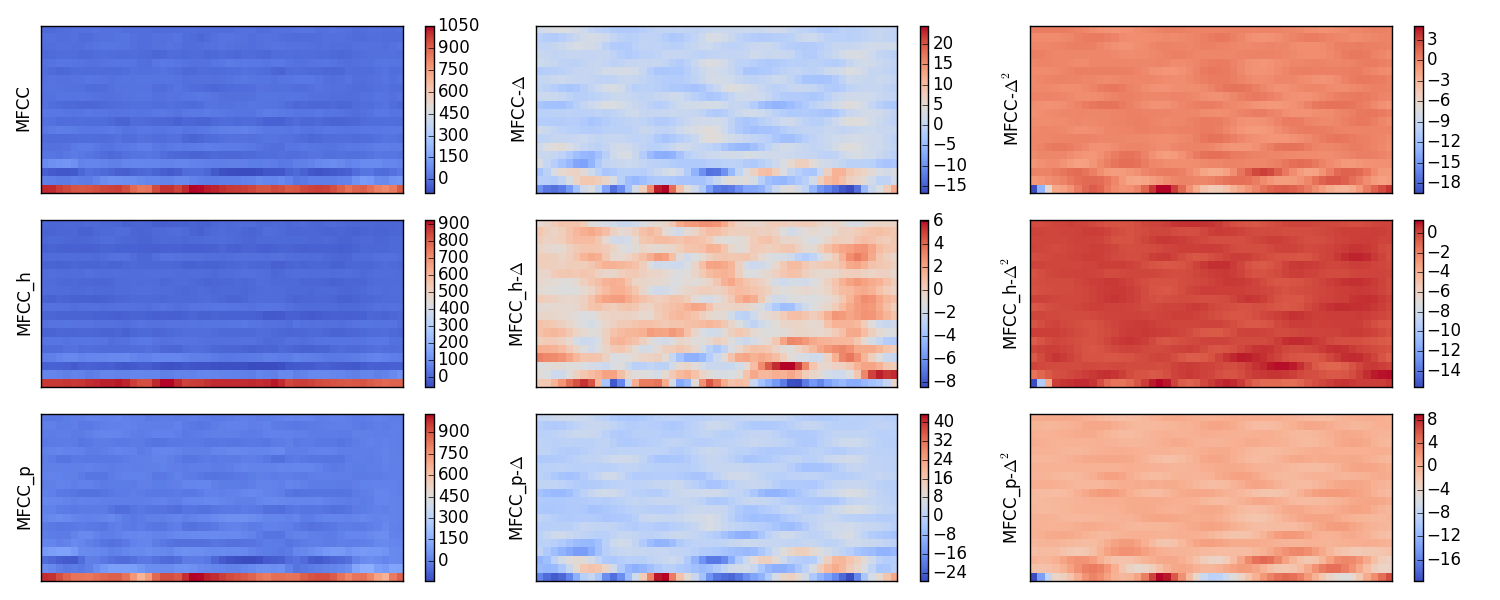
\includegraphics[width=0.7\textwidth]{../fig/HP_deltas1.png}
  \caption{MFCC spectrogram of feature.delta from original clip, harmonic, and percussiv parts}
\end{figure}

\\As metionend in HPSS scattering algorithm for our feature extraction method 3, we performed 2-order HPSS and keep all those MFCC results, which will 14 times more representation points than baseling method. From figure 3.1 we can see all the accuracy representing by color of the points in the search space all turned reddish, which is also confirmed by the significant peak shift between row 1 and row 3 in figure 4.3. Moreover, feature extraction method 3 is even better than method 1 and 2. As we may see from figure 4.3, method 1 and 2 are wider gaussian distribution while the distributin of method 3 is narrower. Furthermore, the peak of method3 is shifted from approximate 60\% in method 1 and 2 to 65\%. In terms of the maximum accuracy, method 3 can have 79\% accuracy while it's 77\% and 76\% in method 1 and 2.

\begin{figure}[!ht]
  \centering
    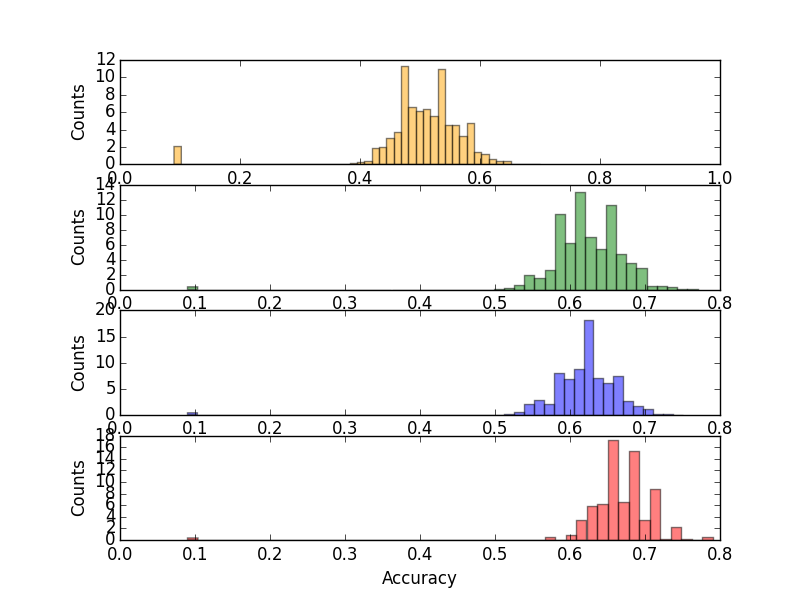
\includegraphics[width=0.7\textwidth]{../fig/histogram_n1.png}
  \caption{Histogram of accuracy result from search space. Top row is baseline method 5, and the remaining rows are new feature extraction method 1, 2, and 3 respectively}
\end{figure}

\begin{table}[h!]
\centering
\begin{tabular}{ l || c | r }
      \hline
      Method Ids & Accuracy (\%) \\ \hline \hline
      Method 1 & 77 \\ \hline
      Method 2 & 76 \\ \hline
      Method 3 & 79 \\ \hline
      \hline
    \end{tabular}
\caption{Methods of each new feature extraction approaches and its corresponding accuracy.}
\label{table:1}
\end{table}

\begin{thebibliography}{10}
\bibitem{fpf} {\sc Low pass filter by FFT convolution}, {\em http://www.dsprelated.com/freebooks/sasp/Example\_1\_Low\_Pass\_Filtering.html}
\bibitem{msc} {\sc Multiscale Scattering for Audio Classifications}, {\em http://www.cmap.polytechnique.fr/scattering/ismir-final.pdf}
\bibitem{dl} {\sc Digital image processing: p067- Dictionary Learning}, {\em https://www.youtube.com/watch?v=XLXSVLKZE7U}
\bibitem{ipm} {\sc Interior-point methods}, {\em https://web.stanford.edu/class/ee364a/lectures/barrier.pdf}
\bibitem{ista} {\sc Iterative Shrinkage/Thresholding Algorithms}, {\em http://people.ee.duke.edu/~lcarin/figueiredo.pdf}
\bibitem{mpwtfd} {\sc Matching pursuits with time-frequency dictionaries}, {\em http://www.cmap.polytechnique.fr/~mallat/papiers/MallatPursuit93.pdf}
\bibitem{eik} {\sc Efficient Implementation of the K-SVD Algorithm using Batch Orthogonal Matching Pursuit}, {\em http://www.cs.technion.ac.il/~ronrubin/Publications/KSVD-OMP-v2.pdf}
\bibitem{mgc} {\sc Music Genre Classification Using Multiscale Scattering and Sparse Representations}, {\em http://www.princeton.edu/~xuchen/resources/pdf/music13.pdf}
\bibitem{data} {\sc GTZAN Music Genre Collection}, {\em http://marsyasweb.appspot.com/download/data\_sets/}
\end{thebibliography}

\end{document}
